% % % % % % % % % % % % % % % % % % % % % % % % % % % % % % % % 
% SPA Project Report Example (Adapted from JPE MSc Diss)
% % % % % % % % % % % % % % % % % % % % % % % % % % % % % % % %
\documentclass[twoside,fontsize=12pt,
     bibliography=totoc, % Include bibliography in contents
     listof=totoc,       % Include lists of figures and tables in contents
     index=totoc,        % Include index in contents
     onehalfspacing      %  or doublespacing 
%     , nopreamble      %  Turn off extended intro material
%     , openright
]{SPAProjectReport}

\usepackage[labelfont=footnotesize,textfont=footnotesize]{caption}   
\usepackage{url}
\usepackage{breakurl}
\usepackage[]{SPAProjectReport}

% Referencing & Bibliography Options - Natbib Package

% Numerical Citing/Referencing Style (uncomment one of these)

% Harvard Style Referencing (Using Authors (Year) labels) 
\usepackage[sort&compress]{natbib}
\bibliographystyle{abbrvnat}       % Harvard Style

% Vancouver Style Referencing (Using numerical labels)
%\usepackage[square, numbers, comma, sort&compress]{natbib}   %
%\bibliographystyle{unsrtnat}

% Astronomy Style Citing - works with NASA ADS
% Uncomment the 3 lines below
%\usepackage[round, authoryear, comma, sort&compress]{natbib}  
%\bibpunct{(}{)}{;}{a}{}{,}    %% natbib cite format used by A&A and ApJ
%\bibliographystyle{abbrvnat-spa}   % Astronomy Style  - Similar to Harvard


%---------------------------------------------------------------------
%\declaration{I hereby certify that this project report, which is
%approximately N thousand words in length, has been written by me at
%the School of Physics and Astronomy, Queen Mary University of London, that all material in this dissertation which is not my own work has been properly acknowledged, and that it has not been submitted in any previous application for a degree.} 

%--Put your information between here----%
\title{A Simple Example SPA Project Report}
\author{Your Name (student number in brackets) }
\supervisor{your supervisor's Name}
\SubmissionDate{\today}

\ModuleName{SPA6776 Extended Independent Project}
\ModuleCredits{30 Credit Units}


%Degree, program or course: ex: Master of Science, Engineering Physics
\Programme{BSc Physics} % The degree, program or course-name goes here
% Uncomment the line below and include your acknowledgments between {}
%\acknowledgements{} 

\newpage% to ensure page 1 starts on front of a page rather than back
%---and here------%

\begin{document}  % -------------------------------------------------

\pagenumbering{roman}
\maketitle
\abstract{Your abstract text goes here.}
\setcounter{tocdepth}{5}
\tableofcontents           % generates Table of Contents
\listoffigures             % generates List of Figures 
\listoftables              % generates List of Tables

\newpage                   % to flush out last roman numeral
\cleardoublepage
\pagenumbering{arabic}     % Set arabic page numbers for main text of report.


\chapter{Introduction}
\label{sec:intro}

This is example content.  It should be replaced with your own.  Its
purpose here is to illustrate basic \LaTeX\ formatting commands.
Chapter \ref{sec:intro} is the Introduction. 
   
\section{A Sample Figure}
Figure \ref{fig:pluto} shows the colour mosaic from the New Horizon's
flyby of Pluto. 
\begin{figure}[hbtp]
  \begin{center}
  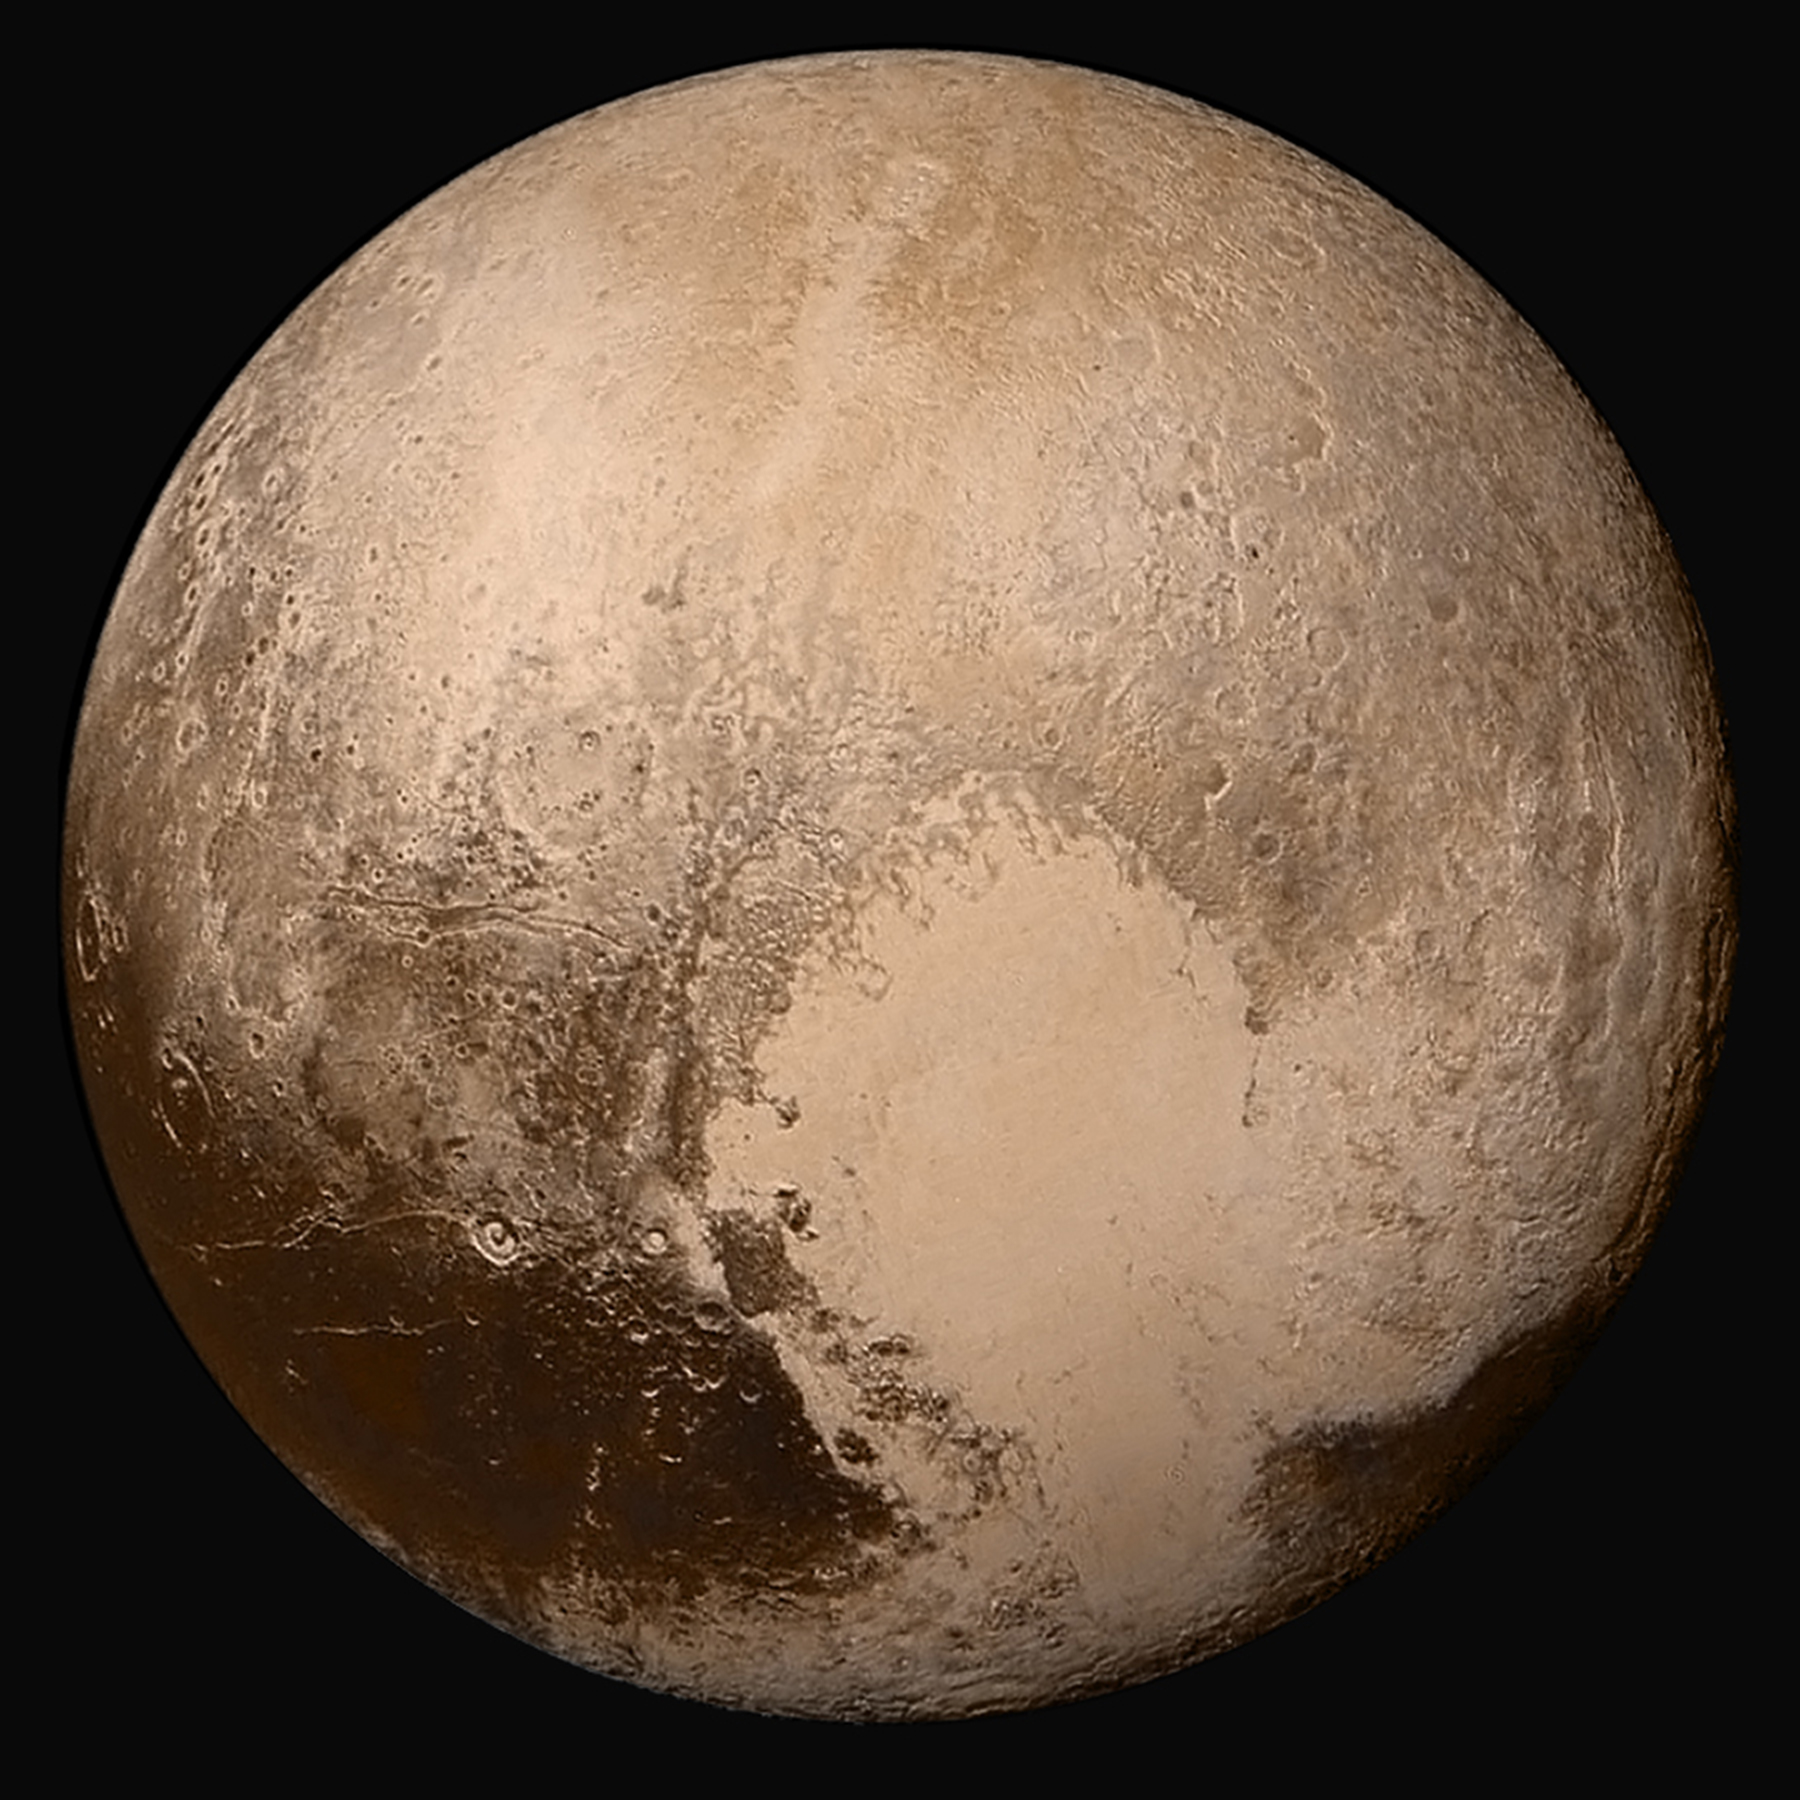
\includegraphics[width=80mm]{diagrams/Example-Image.jpg}  %% file name without extension
  \caption[Example Figure of Pluto]{An example illustrating including figures.  If you're using
    pdflatex you  may use image files in the following formats PDF,
    PNG, JPG or JPEG.  It is probably easiest to store all the files
    in the same directory/folder with your *.tex and *.bib files.} 
  \label{fig:pluto}
  \end{center}
\end{figure}

\subsection{A Sample Equation}
This is how you can include equations.
\begin{equation}
   \label{eq:hydroeq}
   \frac{dP}{dr} = -\rho g(r)
\end{equation}
or inline mathematics such as $E=mc^2$.
By the way, Eq.~\ref{eq:hydroeq} is the relation for hydrostatic balance.

\subsection{Example Citations and References}

You can look on the web for a guide to the \LaTeX\ package natbib and
you will find a host of commands for citing published work.  Here are
a couple examples.

\citet{NHDescription} provides a brief description of the New
Horizons mission to Pluto.

There are many good descriptions of the New Horizons mission to Pluto
\citep[see e.g.,][]{NHDescription}.


%%%%%%%%%%%%%%%%%%%%%%%%%%%%%%%%%%%%%%%%%%%%%%%%%%%%%%%%%%%%%%%%%%%%
%%BIBLIOGRAPHY SECTION
\begin{singlespace}% Start single space for bibliography

\bibliography{references} % The filname here is where all your
                              % bibtex entries go  
\end{singlespace}

\end{document}
